% Template for PLoS
% Version 3.5 March 2018
%
% % % % % % % % % % % % % % % % % % % % % %
%
% -- IMPORTANT NOTE
%
% This template contains comments intended
% to minimize problems and delays during our production
% process. Please follow the template instructions
% whenever possible.
%
% % % % % % % % % % % % % % % % % % % % % % %
%
% Once your paper is accepted for publication,
% PLEASE REMOVE ALL TRACKED CHANGES in this file
% and leave only the final text of your manuscript.
% PLOS recommends the use of latexdiff to track changes during review, as this will help to maintain a clean tex file.
% Visit https://www.ctan.org/pkg/latexdiff?lang=en for info or contact us at latex@plos.org.
%
%
% There are no restrictions on package use within the LaTeX files except that
% no packages listed in the template may be deleted.
%
% Please do not include colors or graphics in the text.
%
% The manuscript LaTeX source should be contained within a single file (do not use \input, \externaldocument, or similar commands).
%
% % % % % % % % % % % % % % % % % % % % % % %
%
% -- FIGURES AND TABLES
%
% Please include tables/figure captions directly after the paragraph where they are first cited in the text.
%
% DO NOT INCLUDE GRAPHICS IN YOUR MANUSCRIPT
% - Figures should be uploaded separately from your manuscript file.
% - Figures generated using LaTeX should be extracted and removed from the PDF before submission.
% - Figures containing multiple panels/subfigures must be combined into one image file before submission.
% For figure citations, please use "Fig" instead of "Figure".
% See http://journals.plos.org/plosone/s/figures for PLOS figure guidelines.
%
% Tables should be cell-based and may not contain:
% - spacing/line breaks within cells to alter layout or alignment
% - do not nest tabular environments (no tabular environments within tabular environments)
% - no graphics or colored text (cell background color/shading OK)
% See http://journals.plos.org/plosone/s/tables for table guidelines.
%
% For tables that exceed the width of the text column, use the adjustwidth environment as illustrated in the example table in text below.
%
% % % % % % % % % % % % % % % % % % % % % % % %
%
% -- EQUATIONS, MATH SYMBOLS, SUBSCRIPTS, AND SUPERSCRIPTS
%
% IMPORTANT
% Below are a few tips to help format your equations and other special characters according to our specifications. For more tips to help reduce the possibility of formatting errors during conversion, please see our LaTeX guidelines at http://journals.plos.org/plosone/s/latex
%
% For inline equations, please be sure to include all portions of an equation in the math environment.
%
% Do not include text that is not math in the math environment.
%
% Please add line breaks to long display equations when possible in order to fit size of the column.
%
% For inline equations, please do not include punctuation (commas, etc) within the math environment unless this is part of the equation.
%
% When adding superscript or subscripts outside of brackets/braces, please group using {}.
%
% Do not use \cal for caligraphic font.  Instead, use \mathcal{}
%
% % % % % % % % % % % % % % % % % % % % % % % %
%
% Please contact latex@plos.org with any questions.
%
% % % % % % % % % % % % % % % % % % % % % % % %

\documentclass[10pt,letterpaper]{article}
\usepackage[top=0.85in,left=2.75in,footskip=0.75in]{geometry}

% amsmath and amssymb packages, useful for mathematical formulas and symbols
\usepackage{amsmath,amssymb}

% Use adjustwidth environment to exceed column width (see example table in text)
\usepackage{changepage}

% Use Unicode characters when possible
\usepackage[utf8x]{inputenc}

% textcomp package and marvosym package for additional characters
\usepackage{textcomp,marvosym}

% cite package, to clean up citations in the main text. Do not remove.
% \usepackage{cite}

% Use nameref to cite supporting information files (see Supporting Information section for more info)
\usepackage{nameref,hyperref}

% line numbers
\usepackage[right]{lineno}

% ligatures disabled
\usepackage{microtype}
\DisableLigatures[f]{encoding = *, family = * }

% color can be used to apply background shading to table cells only
\usepackage[table]{xcolor}

% array package and thick rules for tables
\usepackage{array}

% create "+" rule type for thick vertical lines
\newcolumntype{+}{!{\vrule width 2pt}}

% create \thickcline for thick horizontal lines of variable length
\newlength\savedwidth
\newcommand\thickcline[1]{%
  \noalign{\global\savedwidth\arrayrulewidth\global\arrayrulewidth 2pt}%
  \cline{#1}%
  \noalign{\vskip\arrayrulewidth}%
  \noalign{\global\arrayrulewidth\savedwidth}%
}

% \thickhline command for thick horizontal lines that span the table
\newcommand\thickhline{\noalign{\global\savedwidth\arrayrulewidth\global\arrayrulewidth 2pt}%
\hline
\noalign{\global\arrayrulewidth\savedwidth}}


% Remove comment for double spacing
%\usepackage{setspace}
%\doublespacing

% Text layout
\raggedright
\setlength{\parindent}{0.5cm}
\textwidth 5.25in
\textheight 8.75in

% Bold the 'Figure #' in the caption and separate it from the title/caption with a period
% Captions will be left justified
\usepackage[aboveskip=1pt,labelfont=bf,labelsep=period,justification=raggedright,singlelinecheck=off]{caption}
\renewcommand{\figurename}{Fig}

% Use the PLoS provided BiBTeX style
% \bibliographystyle{plos2015}

% Remove brackets from numbering in List of References
\makeatletter
\renewcommand{\@biblabel}[1]{\quad#1.}
\makeatother



% Header and Footer with logo
\usepackage{lastpage,fancyhdr,graphicx}
\usepackage{epstopdf}
%\pagestyle{myheadings}
\pagestyle{fancy}
\fancyhf{}
%\setlength{\headheight}{27.023pt}
%\lhead{
\includegraphics[width=2.0in]{PLOS-submission.eps}}
\rfoot{\thepage/\pageref{LastPage}}
\renewcommand{\headrulewidth}{0pt}
\renewcommand{\footrule}{\hrule height 2pt \vspace{2mm}}
\fancyheadoffset[L]{2.25in}
\fancyfootoffset[L]{2.25in}
\lfoot{\today}

%% Include all macros below

\newcommand{\lorem}{{\bf LOREM}}
\newcommand{\ipsum}{{\bf IPSUM}}





\usepackage{forarray}
\usepackage{xstring}
\newcommand{\getIndex}[2]{
  \ForEach{,}{\IfEq{#1}{\thislevelitem}{\number\thislevelcount\ExitForEach}{}}{#2}
}

\setcounter{secnumdepth}{0}

\newcommand{\getAff}[1]{
  \getIndex{#1}{MPI,UPENN,NMSA,Leiden,Tube,Wall}
}

\providecommand{\tightlist}{%
  \setlength{\itemsep}{0pt}\setlength{\parskip}{0pt}}

\begin{document}
\vspace*{0.2in}

% Title must be 250 characters or less.
\begin{flushleft}
{\Large
\textbf\newline{Introducing Platform Surface Interior Angle and Its Role in Flake
Formation, Size and Shape} % Please use "sentence case" for title and headings (capitalize only the first word in a title (or heading), the first word in a subtitle (or subheading), and any proper nouns).
}
\newline
% Insert author names, affiliations and corresponding author email (do not include titles, positions, or degrees).
\\
Shannon P. McPherron\textsuperscript{\getAff{MPI}}\textsuperscript{*},
Aylar Abdolahzadeh\textsuperscript{\getAff{UPENN}},
Will Archer\textsuperscript{\getAff{NMSA}},
Igor Djakovic\textsuperscript{\getAff{Leiden}},
Tamara Dogandžić\textsuperscript{\getAff{MPI}},
Li Li\textsuperscript{\getAff{Tube}},
Sam Lin\textsuperscript{\getAff{Wall}},
Jonathan Reeves\textsuperscript{\getAff{Tube}},
Zeljko Rezek\textsuperscript{\getAff{MPI}},
Marcel Weiss\textsuperscript{\getAff{MPI}}\\
\bigskip
\textbf{\getAff{MPI}}Department of Human Evolution, Max Planck Institute for Evolutionary
Anthropology, DeutscherPlatz 6, Leipzig, Germany\\
\textbf{\getAff{UPENN}}Department of Anthropology, University of Pennsylvania, Philadelphia,
PA, USA\\
\textbf{\getAff{NMSA}}The National Museum of South Africa\\
\textbf{\getAff{Leiden}}Department of Archaeology, University of Leiden, Leiden, The Netherlands\\
\textbf{\getAff{Tube}}Department of Early Prehistory and Quaternary Ecology, Eberhard Karls
University of Tübingen, Tübingen, Germany\\
\textbf{\getAff{Wall}}The Wall\\
\bigskip
* Corresponding author: mcpherron@eva.mpg.de\\
\end{flushleft}
% Please keep the abstract below 300 words
\section*{Abstract}
Four ways archaeologists have tried to gain insights into how
flintknapping creates lithic variability are fracture mechanics,
controlled experimentation, replication and attribute studies of lithic
assemblages. Of the these, fracture mechanics has the advantage of being
based more closely on first principles derived from physics and material
sciences, but its practical application to controlled experimentation,
replication and lithic studies more generally has been limited.
Controlled experiments have the advantage of being able to explicitly
quantify the contribution of individual variables to knapping outcomes,
and the results of these experiments have provided models of flake
formation that when applied to the archaeological record of
flintknapping have provided insights into past behavior. Here we attempt
to provide some linkage between fracture mechanics and the results of
the controlled experiments to increase its explanatory and predictive
power. We do this by looking for the impact of the Herztian cone of
percussion, a constant in fracture mechanics, on flake platforms. We
find that the platform width is a function of the Hertzian cone constant
angle and the geometry of the platform edge. This finding strengthens
the foundation of one of the models emerging from the controlled
experiments and with some additional work should make it possible to
merge more of the experimental results into a more comprehensive model.

% Please keep the Author Summary between 150 and 200 words
% Use first person. PLOS ONE authors please skip this step.
% Author Summary not valid for PLOS ONE submissions.

\linenumbers

% Use "Eq" instead of "Equation" for equation citations.
\hypertarget{introduction}{%
\section{Introduction}\label{introduction}}

There is considerable literature dedicated to better understanding how
flakes form. Roughly speaking, this work falls into several broad
categories which we can call fracture mechanics (e.g.~Cotterell and
Kaminga etc., Speth 1972), controlled experiments (e.g.~Speth, Pelcin,
Dibble etc.), replicative experiments (e.g.~Eren etc.), and attribute
analysis of archaeological assemblages. These approaches have each their
own strengths and weaknesses; however, one way to understand the
differences between them is in the directionality of inference. Fracture
mechanics starts with first principles, or laws drawn from physics and
material sciences in particular, concerning how fractures should form in
brittle solids to then make predictions about how flakes should look
(size and shape) under varying conditions (where the core is struck, the
hammer type, how the platform is prepared, the angle of strike, etc.).
To the contrary, controlled and replicative experiments and studies of
actual lithic assemblages look at empirical regularities in size and
shape under varying conditions to build statistical models of flake
formation from which one can try to infer first principles. Both
approaches are, of course, valid and useful, and the relationship
between what is learned from actually doing (experiments) and what is
learned from knowing how it should work in principle (fracture
mechanics) is circular with each informing the other in an iterative
loop.

Understanding first principles causality from statistical modeling,
however, is challenging. McElreath (2018) gives the example of trying to
understand the physics behind race cars by measuring their attributes.
Knowing the speed and handling characteristics of each car, eventually
the right things could be measured on each car to build statistical
models with enough predictive power to know how a new car might perform
in a race, but it would be quite difficult to infer the general physical
concepts (and laws) like torque, angular momentum, friction,
conservation of energy, etc. from these statistical models. Of course,
with prior knowledge of the physics, finding the right attributes to
measure on the cars and statistical modeling are more quickly done. This
is important because even when the physical laws are known, modeling
them directly can be prohibitively complex or computationally expensive
(e.g.~air resistance) whereas experiments and statistical models can
more efficiently arrive at useable solutions.

The same is true of studies of flake formation and the role of fracture
mechanics within it. Fracture mechanics itself is a massive field of
study, but the best examples of its application to flake formation are
from the papers of Cotterell and Kamminga () and of Speth (1972). These
papers start with the physics of fracture mechanics in brittle solids to
then explain how flakes are formed and, therefore, why they vary. Some
aspects, like the bulb of percussion, are more easily directly accounted
for in fracture mechanics whereas for other attributes, like flake size
and shape, the conceptual and mathematical frameworks are provided.
However, as with the just mentioned example of air resistance,
translating the physics of how flakes are formed into a workable model
that can predict flake size and shape given the relevant parameters
(e.g.~core shape, angle of blow, force of blow, etc.) has not come to
pass (cf.~Speth 1972), and it may not come to pass any time soon.
{[}give example of age of the known universe fracture mechanics
model{]}.

So instead, while some papers in controlled experiments in flake
formation may cite papers from fracture mechanics, their approaches are
all based on statistical modeling. Speth's work on this topic makes a
good example. His 1972 paper uses fracture mechanics to derive a formula
to predict flake size which is then tested against a set of actual
flakes from a prehistoric site. By 1975 and again in 1981, Speth had
moved to experimental approaches (ball bearings on glass) and the
connection back to fracture mechanics had all but disappeared. Dibble
goes further and simply dismisses fracture mechanics from the start as
nearly irrelevant (Dibble and Whittaker 1981). Instead of looking to
fracture mechanics for insights into what to study, experimental studies
are being informed by replicative knappers and observations on how
actual lithic assemblages vary. Dibble is explicit in stating that his
experimental research is based on what knappers would have been able to
control (Dibble and Whittaker 1981; Dibble 1997). Coming back to the
race car analogy, we are carefully building cars controlling for engine
size, wheel configurations, foils, etc., things that are generally
thought to be important for making a car go fast, and then measuring
their speeds. Again, though, because it is also difficult to go in the
other direction (from statistical modeling to first principles), the
controlled experiment papers have not produced a general model of how
flakes form. Instead, we have a series of statistical models that are
difficult to relate to one another. The strongest and most influential
of these is the EPA-PD model.

The EPA-PD model states that flake size (mass) is primarily a function
of two important variables: exterior platform angle (EPA) and platform
depth (PD). Increasing either increases flake size, but the relationship
between the two is geometric such that at higher values of EPA changes
in PD have a greater effect on flake size. The EPA-PD model has been
replicated in multiple experiments (Dibble and Whittaker 1981; Dibble
and Pelcin 1995; Speth 1975, 1981), is known to work across raw material
types (Dogandzic et al.~2010), is known to work in actual lithic
assemblages (Dibble 1997), and is argued to have a stronger effect on
flake size and shape than does core surface morphology (Pelcin 1997;
Rezek et al.~2011). The EPA-PD model of flake formation, however, has
some weaknesses. For instance, beveled flakes, where the area behind the
platform is thinned, are not easily included into the model (Leader et
al.~2017). Beveled flakes are typically larger (mass) than the EPA-PD
models predicts given their lower platform depths. The EPA-PD model also
does not explain why flake size and shape change with varying angles of
blow (Magnani et al.~2014), and it does not account for flake width,
which is obviously a major component of shape. It is also worth noting
that while the percentage of variability in mass explained by the EPA-PD
model is typically high in the Dibble glass experiments, it is far lower
in actual lithic assemblages. It is low enough that its utility for
measuring retouch intensity (i.e.~knowing how much mass has been removed
from a flake through retouch) is limited (Dogandzic PLOS One), and so
there have been various proposals to improve the statistical modeling of
flake mass from different sets of measures (Braun et al.; Dogandzig et
al.; Archer et al.). Again, though, it is not really clear why one
measurement technique should work better than another, and success is
measured by R2 values (e.g.~Muller and Clarkson; Archer). The problem is
that we still do not know really how flake formation works in a way that
translates to measurable attributes.

Here we propose to build on the EPA-PD model by 1) switching the focus
from variables controlled by the knapper to variables that might be more
directly related to flake initiation and formation and by 2) drawing
insights from the fracture mechanics literature in doing so. In
particular, we start with the proposal that Hertzian cones, a constant
in percussive fracture mechanics, have a measurable impact on where the
fracture initiates, and this in turn plays an important role in
determining flake size and shape. We model this proposal as follows.
When a core is struck, the fracture initially travels from the point of
percussion at a fixed angle that corresponds to the Hertzian cone angle.
This angle has been measured in glass at 68.5 degrees or 137 across the
full cone (Roesler 1956) and is similarly reported to be 136 degrees in
Cotterell and Kaminga (1987). Importantly, this angle varies only with
raw material type (). Changing the type of indenter (hard versus soft
hammer), the size of the indenter, or the force with which the material
is struck do not change the cone angle (). Changing the angle of blow
likely changes the orientation of the cone, but it does not change its
angle (). When the fracture, spreading at this constant angle,
encounters the core surface a fracture plane forms roughly parallel to
the core surface (in other words at an angle roughly equivalent to the
EPA). At this point the importance of the Hertzian cone angle quickly
diminishes, and our model no longer applies. While we are unsure where
exactly the Hertzian cone will first intersect the core surface, we take
as our proxy of this model the location where it initiates on the
platform edge (where the platform meets the core surface), and we
measure the angle between the point of percussion and these two points.
This angle we term the platform surface interior angle or PSIA, and our
prediction is that this angle is a constant that directly follows from
the Hertzian cone constant. If this model is correct, then it means that
platform width is determined by the geometry of the platform edge in
relation to where the core is struck. In this way, platform width is
integrated into the EPA-PD model, and how PD actually impacts flake size
becomes based in fracture mechanics. Additionally, this model is not
without behavioral implications in that it could explain how the
manipulation of the platform impacts the size and shape of flakes.

To test this model, we examine several sets of flakes, including flakes
produced in the Dibble glass experiments and flakes from replication
experiments, using several methods to measure the platform surface
interior angle. We find that mean angle in all datasets, regardless of
how it is measured, is the same (approximately 136 degrees) and quite
consistent with above mentioned values for Hertzian cone formation
(Cotterell and Kaminga 1987). There is some variability in the platform
surface interior angle, and it is clear that this variability cannot be
solely attributed to measurement error. In the Dibble glass experiments,
where key variables are controlled, there is some indication that the
platform surface interior angle responds to the angle of blow. Our
finding is consistent with all of the empirical results of the Dibble
experiments and it explains some of the patterns in those data that
previously were unaccounted for. When platform surface interior angle is
combined with exterior platform angle, we may have a model for flake
formation that can explain a larger portion of the variability we see in
stone tool assemblage and that may allow for a closer link to
predictions coming from fracture mechanics.

\hypertarget{materials-and-methods}{%
\section{Materials and Methods}\label{materials-and-methods}}

We examine the platform surface interior angle in three different
datasets. First, we examine glass flakes and cores coming from the
Dibble controlled experiments in flake formation (Dibble and Rezek
2009). This dataset has the advantage that a number of potentially
important variables are either controlled for or measureable. These
include the exterior platform angle, the angle of blow, the hammer type,
material knapped, and metrics such as platform thickness, platform
width, flake length, width and thickness, and flake weight. Hereafter
this dataset if referred to as the Dibble glass data. Second, we attempt
to validate the findings from the Dibble glass data by measuring the
platform surface interior angle in a large set of flakes coming from
replicative experiments. These flakes were made by so and so and so and
so with the intent of replicating various core reduction strategies from
the initial formation of the core through to flake production and core
maintenance. For each of the flakes coming from these reduction series,
the technology and the type of hammer (hard hammer, soft hammer and
indirect percussion) are known. Hereafter this dataset is referred to as
the Campagne data (see Archer et al.~2020 for additional details on the
structure of this dataset). Third, in addition, we measured a small set
of flakes produced at the Max Planck Institute in Leipzig, Germany, in
the context of teaching, replication, and experimentation. In this case,
no details are known about how the flakes were produced, and this set of
flakes is used here only to test a method for measuring the platform
surface interior angle. One of us (SPM) selected flakes from boxes of
debris. Every effort was made to avoid bias, and all flakes with
complete platforms and measurable platform widths were retained.
Hereafter this dataset is referred to as the MPI data.

The methods used to measure the platform surface interior angle varied
substantially between the three datasets. First, for the Dibble glass
data, we used the following procedure. Dibble used several core forms,
but the first and most common type is what he called the semispherical
core. This core (reproduced here) looks like a loaf of bread with flat,
squared off sides and back, and a curved or domed flaking surface. An
unworked example of this core type was scanned using an XX surface
scanner. The resulting mesh was then processed in R to rotate the
platform to be perpendicular to the Z axis (or coincident with the XY
plane). The XY coordinates of the triangles forming the platform were
then extracted from this model and a convex hull fit to this cloud of
points to have the full outline of the platform on the Dibble
semispherical cores (Figure 1). Next, we extracted just the portion of
the outline that is where flakes are struck from these cores, and we fit
a polynomial curve to these points. Using the formula for this curve, we
created a series of equally spaced (in X) points along the platform edge
(see (see Figure 1). We then filtered Dibble's glass data to have only
flakes made from the semispherical cores by hard hammer. We include only
flakes with a feather termination, and we exclude flakes coming from
experiments on platform beveling and so-called `on-edge' core strikes.
Knowing that Dibble tried to strike flakes from these cores at the
center or peak of the core surface curvature, we use the platform depth
reported for these flake to position the point of percussion relative to
the set of platform edge outline points described above. Next, working
back from the platform edge, the locations left and right of the point
of percussion and on the platform edge points that yields a platform
width equal to the reported platform width for that flake is determined.
Finally, the platform surface interior angle is calculated (arc-cosine
of the dot product of two normalize vectors) as the angle between the
two line segments formed by the left platform width point and the point
of percussion and the right platform point and the point of percussion.

{[}I will insert a new figure showing a Dibble glass core and how the
measures we talk about here are made{]}

\begin{figure}
\centering
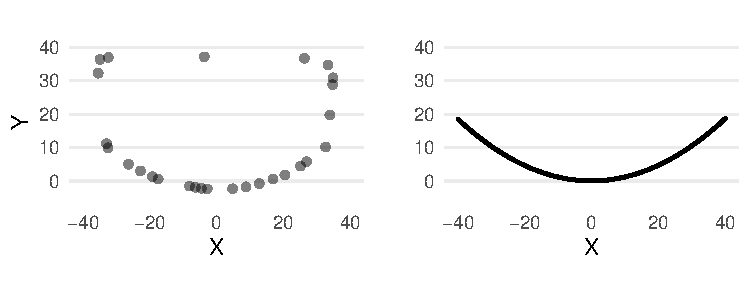
\includegraphics{PSIA_Manuscript_files/figure-latex/fig1-core_outlines-1.pdf}
\caption{Outline of Dible core surface (left) and the polynominal fitted
to the core edge (right).}
\end{figure}

We note that there are several potential sources of error in this
method. First, we are assuming that each flake is struck from the center
of the core, and while this was the intention in the Dibble experiments,
there is certainly some error associated with this. Second, we are
assuming that the flake removal is centered on the center of the core
and parallel to the core surface (i.e.~that it is not twisted to one
side or the other). To the extent that either of these assumptions is
invalid, it will impact the angle calculation. {[}could simulate this to
get an idea of the error{]}

To verify the angles computed in this way from the Dibble glass data, we
also measure this angle directly on a subset of these flakes. We use two
techniques for this measurement to begin to test how to measure the
platform surface interior angle as part of more traditional lithic
attribute measures. In the first method, we measure the three sides of
the triangle formed by the two platform width points and the point of
percussion using digital calipers precise to .01 mm {[}check this{]}.
Using standard trigonometric formulas, we then calculate the interior
angle of this triangle that corresponds to the platform surface interior
angle as described above. In the second method, we use a digital
goniometer precise to XX degrees {[}check this{]} to record this angle.
The joint of the goniometer is positioned at the point of percussion and
the jaws positioned to cross the two platform width points. Both of
these methods come with possibilities for error. Both are impacted by
one ability to pinpoint the point of percussion. In the Dibble glass
flakes, because the core edge is standardized, identifying the the two
platform width points is fairly straightforward. However, in the
goniometer method, taking the measurement to these points while avoiding
the curvature of the bulb of percussion is not without some
difficulties.

Second, for the Campagne data, we use the following procedure. All of
the flakes were scanned using an Artec surface scanner. Each of the
flake meshes was then landmarked (see Archer et al.~2020 for additional
details on the scanning and landmarking). For our purposes, three of
these landmarks are important: the two points (left and right) where the
interior platform intersects the core surface (the platform width) and
the point of percussion. These three points are homologous with the
three points described above for computing the platform surface interior
angle. This angle, therefore, can be once again computed as the dot
product of these two line segments. However, there is an important
difference in that with the Dibble glass data all computations are with
two dimensional line segments and in the Campagne dataset the line
segments are in three dimensions. In the latter case, the angle is
computed in a two dimensional plane that is coincident with both line
segments, but we note this difference because it could introduce a
certain amount of incomparability in the two datasets. Our expectation
is that these angles could average larger than the Dibble glass data
because, for instance, lifting the point of percussion relative to the
two platform points would result in a larger platform surface interior
angle.

Third, for the MPI data, we use only the goniometer method described
above. One of us (MW) made the measurements with instructions only on
the mechanics of the measurement. To avoid bias, MW was given no prior
knowledge of the results of the previous studies outlined above or of
how platform surface interior angle may function in flake production. In
the course of measuring the flakes, several problematic platforms were
identified where the measurement of the platform surface interior angle
was not as clear as the person selecting the flakes (SPM) had initially
believed. These flakes were removed from the analysis.

We use the R () statistical environment to do this analysis. This paper
is an rMarkdown document, and it is included in the supplementary
information along with the data files needed to compile the document and
replicate all of the figures, tables, and statistics.

\hypertarget{results}{%
\section{Results}\label{results}}

\begin{figure}
\centering
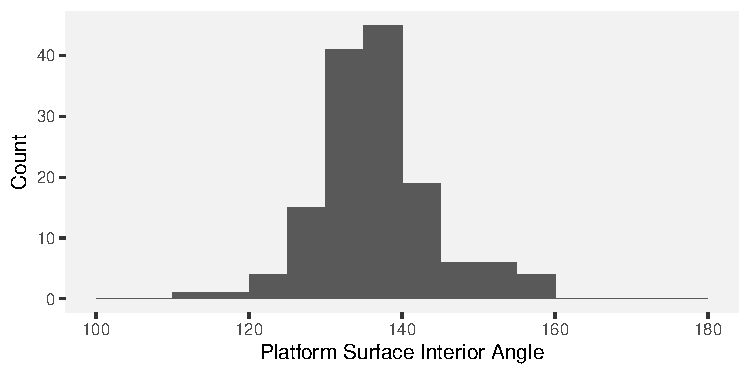
\includegraphics{PSIA_Manuscript_files/figure-latex/fig2-test_1_angles-1.pdf}
\caption{Distribution of estimated platform surface interior angles
(PSIA) based on the Dibble glass flakes.}
\end{figure}

Figure 2 shows the distribution of platform surface interior angles in
the Dibble glass dataset. The distribution has a mean of 136.49±7.56.
Variation in this angle does not seem to be related to platform depth,
exterior platform angle or mass (Figure 3). There is a relationship
between platform width and the platform surface interior angle such that
larger angles result in wider platforms (see Figure 3).

\begin{figure}
\centering
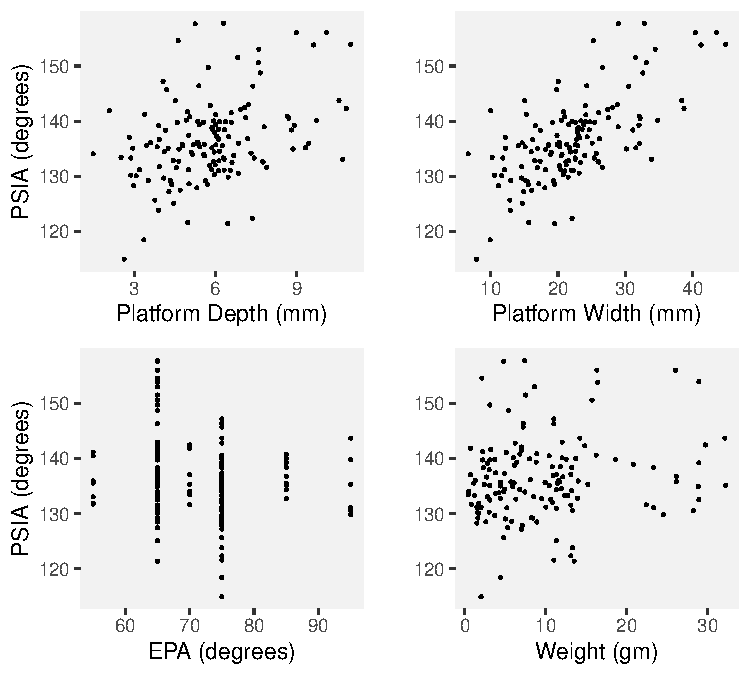
\includegraphics{PSIA_Manuscript_files/figure-latex/fig3-angles_to_other_measures-1.pdf}
\caption{PW, PD, EPA and mass against the estimated platform surface
interior angles based on the Dibble glass flakes.}
\end{figure}

There also appears to be a relationship between the angle of blow and
the platform surface interior angle (Figure 4). While there are fewer
cases with angles of blow less than 20, there is some indication in the
data that lower angles of blow are correlated with lower platform
surface interior angles. After an angle of blow of between 10-20
degrees, however, the angle of blow is not correlated with the platform
surface interior angle.

\begin{figure}
\centering
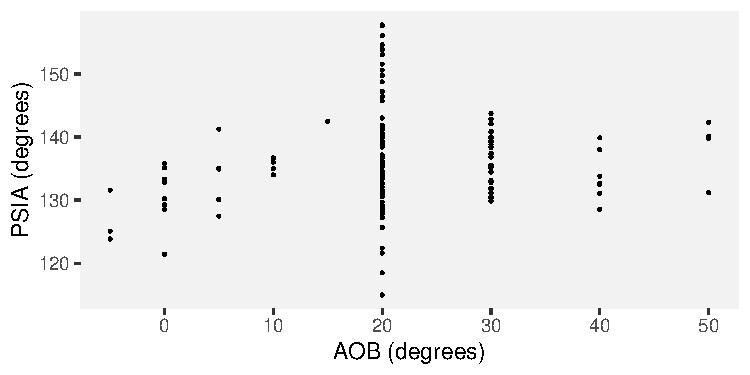
\includegraphics{PSIA_Manuscript_files/figure-latex/fig4-AOB_to_PSIA-1.pdf}
\caption{AOB against the estimated platform surface interior angles
based on the Dibble glass flakes.}
\end{figure}

Another way of looking at the relationship between platform width and
platform surface interior angle is to calculate what the platform width
would be if the platform surface interior angle is a constant and
compare this to the actual platform width. We can do this by placing the
point of percussion on the same platform outlines as above using the
known platform depth for each of the flakes in the Dibble glass data
set. We then use the average platform surface angle computed above to
extend two vectors from this point of percussion to the platform edge.
Where these vectors intersect the platform edge defines the left and
right limits of the platform width. This estimated value is then plotted
against the actual, measured platform widths (Figure 5).

\begin{figure}
\centering
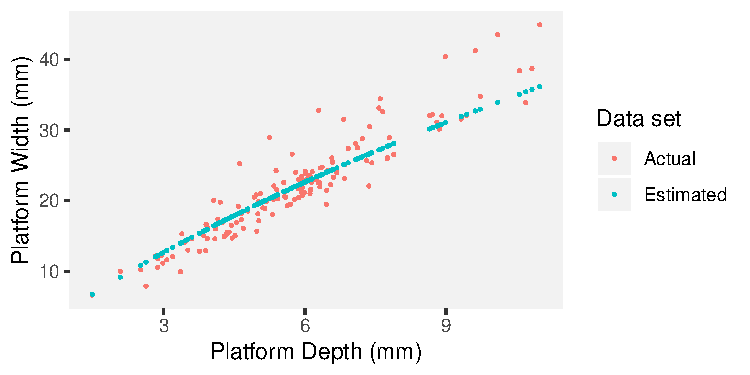
\includegraphics{PSIA_Manuscript_files/figure-latex/fig5-pd_pw_with_estimated_pw-1.pdf}
\caption{The actual platform depth to platform width data from the
Dibble glass core flakes and the estimated platform width using the
average platform surface interior angle calculated previously.}
\end{figure}

Figures 6 and 7 show comparisons of the results of the estimated
platform surface interior angle presented above with direct measurements
of this angle on a sample of 49 of the Dibble glass flakes. For this
sample, the platform surface interior angle is 135.71±4.86. When
measured with a digital goniometer the angle is 133.44±4.61, and when
measured with digital calipers and calculated using trigonometry the
angle is 135.86±8.85.

\begin{figure}
\centering
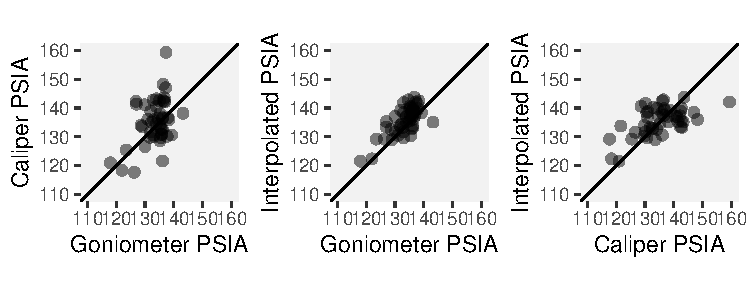
\includegraphics{PSIA_Manuscript_files/figure-latex/fig6_remeasure_comparisons-1.pdf}
\caption{A comparison of the interpolated platform surface interior
angle, this same angle as calculated from caliper measurements, and this
same angle measured with a goniometer. All measures are in degrees.}
\end{figure}

\begin{figure}
\centering
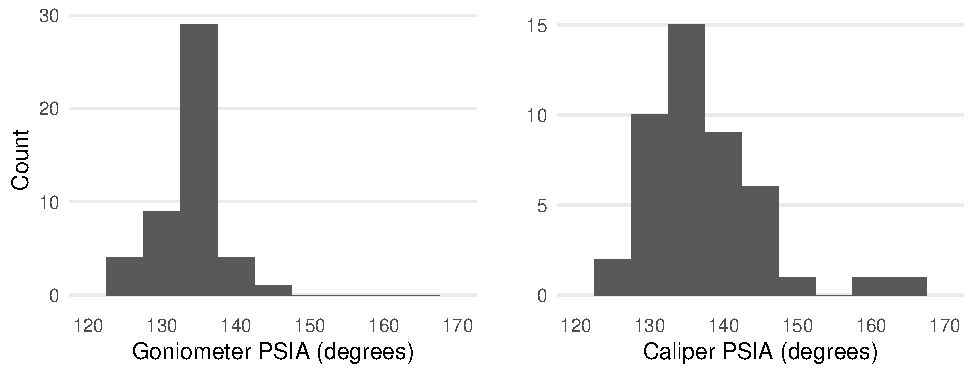
\includegraphics{PSIA_Manuscript_files/figure-latex/fig7_remeasure_distributions-1.pdf}
\caption{The distributions of platform surface interior angle as
directly measured with a goniometer and as calculated from caliper
measurements.}
\end{figure}

The distribution of the platform surface interior angles for the 568
flakes in the Campagne dataset is shown in Figure 8 with color coding
for the type of percussion technique. Here the mean platform surface
interior angle for all flakes is 138.63±13.27. Punch flakes have a lower
platform surface interior angle (stats), and soft hammer flakes have a
mean of XX. When we look at only the hard hammer flakes, which is the
technique used in the Dibble glass dataset, the mean platform surface
interior angle is 140.36±12.38.

\begin{figure}
\centering
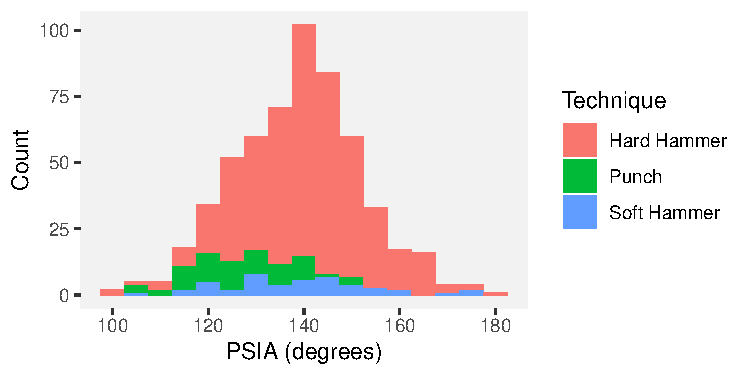
\includegraphics{PSIA_Manuscript_files/figure-latex/fig8-camp_angles-1.pdf}
\caption{Distribution of platform surface interior anglesin the
Campaigne data set color coded by percussion type.}
\end{figure}

In the Campagne data, platform surface interior angle does not covary
with platform width, platform thickness or the shape of the platform (as
measured by the ratio of platform width to platform depth). Though
sample size is perhaps a problem, there is perhaps an indication that
for larger platform depths, there is less variability in the platform
surface interior angle.

\begin{figure}
\centering
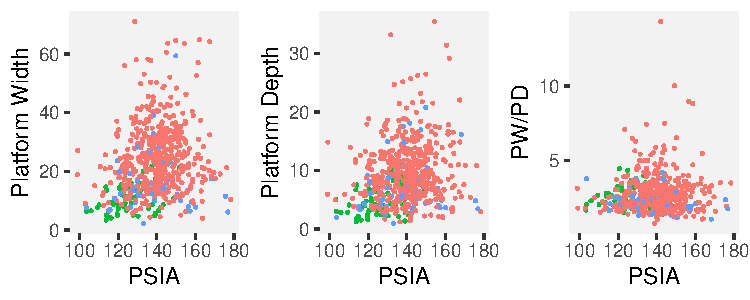
\includegraphics{PSIA_Manuscript_files/figure-latex/fig9-PSIA_to_other_measaures-1.pdf}
\caption{Platform surface interior angle as a function of platform
width, platform depth, and EPA in the experimental flake collection.
Color coding is the same as in Figure 8.}
\end{figure}

The distribution of platform surface interior angles in the MPI dataset
as measured by a digital goniometer is presented in Figure 10. This
dataset contains \texttt{67} flakes, and the mean is 137.75±10.97, in
keeping with the other datasets.

\begin{figure}
\centering
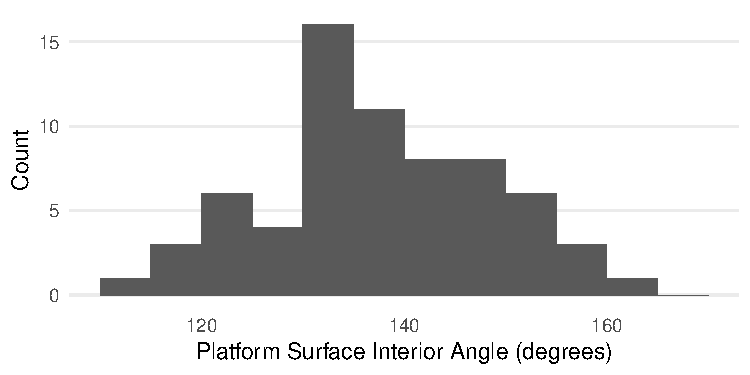
\includegraphics{PSIA_Manuscript_files/figure-latex/fig10-mpi_data-1.pdf}
\caption{Distribution of platform surface interior angle in the MPI
flakes dataset as measured by a digital goniometer.}
\end{figure}

\hypertarget{discussion}{%
\section{Discussion}\label{discussion}}

Each of the datasets and measurement systems used to determine the
platform surface interior angle yielded very similar results, and these
results are consistent with the prediction based on the already known
and constant angle of Hertzian cones (136-137 degrees). These results
pull platform width directly into the EPA-PD model of flake formation,
but they also suggest that this model needs to be nuanced a bit. All
other things being equal, in the PSIA model what determines the size of
the flake is how far into the core it is struck. The deeper into the
core the flake is struck, the greater the width will become because of
the constant platform surface interior angle and the thicker the flake
becomes as well. However, and this is the nuance, while platform
thickness is normally a good proxy for how far into the core the flake
is struck, it is not the same thing. Beveled flakes illustrate why this
is true.

Beveled flakes are ones where material is removed behind the platform
prior to striking the core. Dibble recognized that beveling altered the
EPA-PD model of flake formation such that the interaction of platform
depth and exterior platform angle no longer predicted flake size (Leader
et al.). Beveled flakes have too thin a platform for their size.
However, the inclusion of platform surface interior angle pulls beveled
flakes back into the model. Too illustrate this point, we examine some
of the beveled flakes in the Dibble glass dataset.

In the Dibble glass dataset there are 11 beveled flakes coming from
semispherical cores and otherwise conforming to our selection criteria.
They are plotted in Figure 11 along with the non-beveled flakes to
illustrate how the beveling changes the relationship of platform
thickness to platform width. For a given platform width, the beveled
flakes have much shallower platforms (smaller PD) than expected. To
illustrate the power of platform surface interior angle to explain these
flakes, we can build a linear model to predict platform thickness from
the platform surface interior angle and platform width on the
non-beveled flakes in the Dibble glass dataset. We then use this model
to predict the platform thickness of the beveled flakes. However, the
platform surface interior angle is not known for these flakes, and so we
substitute the average PSIA in its place. When this is done, the
platform thickness for the beveled flakes plot on the same trend line as
the non-beveled flakes (see Figure 11).

This reconstructed platform depth can then be used to improve the EPA-PD
model to give better estimates of flake size. The main aspect of size
that Dibble et al.~have focused on is weight, and so we model flake
weight as a function of EPA, platform depth and the interaction of the
two (see Figure 11). The cube root of weight is used to correct for the
different dimensions in the model. Next, we use this same model to
predict flake weight in the beveled flakes using the platform depth as
originally measured on these beveled flakes. In this case, the predicted
flake weights are much too low (see Figure 11). Finally, we use the
modeled platform depth, as calculated above, to predict flake weight
again using the non-beveled flake model. In this case, the flake weights
plot in among the rest of the non-beveled flakes (see Figure 11). Thus
the beveled flakes are the correct size when we think of PD in the
EPA-PD model not as a measure of platform depth but rather as a measure
of how far into the core the flake is struck, which then determines the
flake width via the platform surface interior angle and the platform
shape. Beveling does not change the expected size of these flakes when
flake formation is viewed this way.

\begin{figure}
\centering
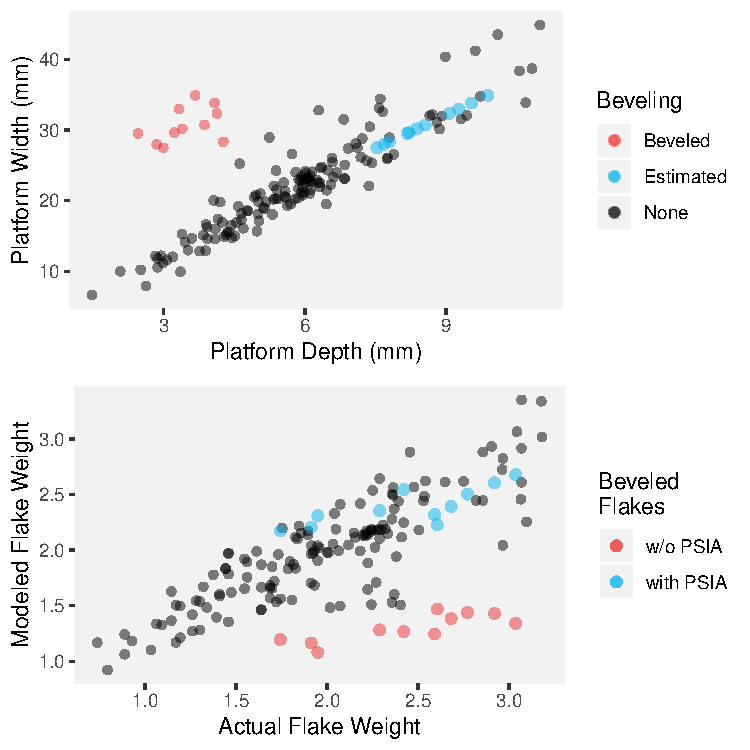
\includegraphics{PSIA_Manuscript_files/figure-latex/fig11-bevel_with_estimated_pd-1.pdf}
\caption{Platform depth to platform width including beveled flakes
(left). Estimated points are the beveled flakes with recalculated
platform depths based on the average PSIA and their actual platform
width. To the right, the actual flake weight is compared to the
predicted flake weight based on an EPA-PD model for non-beveled flakes.
The predicted weight using the actual (w/o PSIA) and the modeled (with
PSIA) platform depths for the beveled flakes are then plotted as well.}
\end{figure}

There is some indication in the Dibble glass data that the angle of blow
may impact the platform surface interior angle. At low angles of blow
(perpendicular to the core surface) the platform surface interior angle
is below average, and it appears to increase until an angle of between
10 and 20 degrees (from perpendicular) after which the platform surface
interior angle remains essentially unchanged. With the caveat that the
Dibble glass data set has very few cases with angles of less than 20
degrees, the fracture mechanics literature suggests a relationship like
this. The angle of blow changes the direction, though not the size, of
the Hertzian cone such that flakes struck from cores with a high angle
of blow (oblique strike) should have ``steeper and less prominent cones
and less salient bulbs of percussion than flakes which are struck more
steeply {[}or more perpendicular{]}'' (Speth 1972:38). Experimentally,
however, Magnani et al.~(2014) seem to find the opposite. They report
that a negative angle of blow (here values less than 0 meaning a strike
directed into the core rather than towards the core surface) have
smaller bulbs relative to the weight of the flake. In our Campagne data
set, we see a difference between flakes made from direct hard-hammer
percussion and those made with a punch technique. The latter cluster at
the low range of platform surface interior angles. This difference could
be interpreted as reflecting a difference in the angle of blow in that
punch flakes are more likely to be struck perpendicularly to the
platform surface. More work needs to be done, in particular analyzing
Dibble glass data set where angle of blow is well controlled, but we
suggest that increasing the angle of blow has the effect of tipping the
direction of the Hertzian cone such that it intersects the core surface
not as a circle but rather as an ellipse. Thus while the angle of the
cone itself remains unchanged, its intersection with the surface
broadens and results in higher platform surface interior angles. Thus,
if this model is correct, striking a core with a high angle of blow will
result in a larger platform width for a given platform thickness.

The direct measurement of platform surface interior angle in a subsample
of the Dibble glass flakes shows that our method for finding this angle
using the core morphology and platform depth is working. However, there
is variability in this angle depending on how it is measured. In general
it seems that the direct measurement with a goniometer performs better
than the indirect calculation of the angle from three caliper
measurements. Of the two systems, the caliper measurements show greater
variability than do the goniometer measurements. The caliper method can
also fail completely when measurement error produces a triangle with
impossible side lengths (e.g.~the sum of the two shorter sides does not
equal the length of the longest side). Importantly too, this is only
knowable once the measures are taken and an angle is calculated, making
it much more difficult to correct, whereas the goniometer method
produces an angle each time. Our study, however, does not indicate which
of the three methods in this case is correct, nor do we know the error
associated with any of these methods. Now that platform surface interior
angle seems to produce results relevant to understanding flake
formation, additional studies are required to better know the error
distribution on an individual measure. We note too that this error
distribution will likely vary with the angle itself, the size of the
point of percussion, and other factors that remain to be identified. The
question, however, is whether this measurement error will overwhelm
patterns, for instance, showing a potential correlation in angle of blow
and platform surface interior angle. It is our expectation that with a
digital goniometer, direct measurement of the platform surface interior
angle can become a standard measurement within an attribute analysis,
but this remains to be determined.

We note that our finding that the platform surface interior angle varies
around a constant derived from fracture mechanics appears to be
consistent with all of the findings to date of the Dibble glass
experiments (). Additionally, it perhaps helps explain or account for
one of the more counter intuitive findings of the glass experiments,
namely that flake size (mass) is not impacted by the force with which
the core is struck (Dibble and Rezek 2009). In the EPA-PD model, the
amount of force required to remove a flake given a particular
combination of EPA-PD is a constant. Subtracting force means that the
flake is not initiated. Adding force does not change the shape (size and
mass) of the resulting flake. This makes sense in the PSIA addition to
the model. In fracture mechanics, it is known that striking a material
harder does not change the angle of the Hertzian cone. It will change
the size of the cone but not the angle. Thus when a core is struck, how
far into the core the Hertzian cone can travel will be a function of
force, but where it is destined to intersect the core surface does not
change. So striking a Dibble glass core harder at a particular point
does not change the platform width, and as a result, the subsequent
fracture plane that removes the flake has much less freedom to change
the size of the flake.

\hypertarget{conclusions}{%
\section{Conclusions}\label{conclusions}}

Fracture mechanics is a massive field of study with both great potential
and great difficulties for understanding flake formation. The potential
is that the physical laws and models coming from fracture mechanics are,
ultimately, how the actions of knappers are translated to usable flakes.
The difficulties are both inherent to the field itself and the
complexity of the problem (some solutions require more time and
computing power than exists) and relate to the challenges of
interdisciplinary work where the equations and goals of one field are
terribly difficult to bring into another. This later point is clearly
seen in the early fracture mechanics literature and the minimal impact
it has had on experimental and replicative studies of flake formation.

This said, our goal here was to return to this literature and to try to
find some useful insights that could be translated to a better
understanding of the underlying mechanisms (or first principles) of
flake formation and that might thereby lead to a better integration of
the various statistical models currently in use. To do this, we
discarded the existing focus in the experimental literature on what
knappers do and instead focused on attributes that may be more directly
related to fracture mechanics. Thus we focused our attention on the
Hertzian percussion cone as a constant and wondered if it could help
explain platform width, an aspect of flake size and shape that up to now
has been absent from the dominant EPA-PD model of flake formation. We
measured three different collections in multiple different ways and
found that in each case the angle formed by the platform width and the
point of percussion to be, on average, essentially the same as what is
predicted from fracture mechanics for the angle of the Hertzian cone.

We conclude that the platform surface interior angle is an important
determinant in flake size and shape. While it would seem that it is a
constant and not under direct control by the knapper, the knapper is
exploiting the properties of this angle when preparing the platform and
its contact with the platform surface and when deciding how far into the
core to strike. In our model, this is how the PD side of the EPA-PD
model of flake formation is translated into a flake of a particular size
and shape. In other words, it is not the PD that directly structures
flake size but rather PD is proxy for how far into the core a flake is
struck which then, through the platform surface interior angle,
structures the size and shape of the flake.

This, however, requires further testing, particularly with beveled
flakes where PD performs poorly as a proxy for how far into the core a
flake is struck. If the platform surface interior angle performs better
in these circumstances, then we will have improved the EPA-PD model and
helped to integrate what are now disparate studies (Dibble and Rezek
2009 and Leader et al.). Additionally, while our study shows that the
average platform surface interior angle conforms well to predictions
from fracture mechanics, it is still clear that there is variability
around this mean. Given that there is certainly some chaos in flake
formation, we are not sure how much variability to expect. {[}something
about the glass cores versus the flint flakes{]} However, it is also
clear that the model does not work at all for some flakes. We would like
to propose that these flakes are not formed by percussion flaking (need
to revisit the Cotterell papers and bending flakes, versus percussive
flake vs.~one other category) and that alternative models will be
required in these cases. Clearly more data are required to begin to
understand which kinds of flakes fail the platform surface interior
angle model, but these flakes should in turn allow us additional
insights into flake formation.

\hypertarget{acknowledgements}{%
\section{Acknowledgements}\label{acknowledgements}}

The knappers in Campagne. We thank the Max Planck Society for funding
portions of this work. SPM, MW, WA, ZR and TD thank Jean-Jacques Hublin
for his support this research agenda. Sadly Harold Dibble died before
the main findings of this paper were discovered. However, without his
vision and his efforts to build a data set of flakes made under
controlled conditions, this paper would not have been possible. We
dedicate this paper to him.

\hypertarget{references}{%
\section{References}\label{references}}

\nolinenumbers


\end{document}

